	\chapter*{Anexo 3 Instalación Eclipse ADT} % si no queremos que añada la palabra "Capitulo"
	\addcontentsline{toc}{chapter}{Anexo 3} % si queremos que aparezca en el índice
	\markboth{Anexo 3}{Anexo 3} % encabezado
	
		En este anexo voy a explicar como se debe instalar Eclipse ADT con SDK de Android en la versión r20, versión que he usado para el desarrollo de la aplicación móvil MotoSafe.
		
		Los tres pasos fundamentales a seguir para tener el entorno de desarrollo instalado en nuestro ordenador son los siguientes:
		
		\begin{itemize}	
			
			\item Descargar Android SDK.
			
			\item Descargar las últimas herramientas del SDK y plataformas desde el Manager del SDK.
			
			\item Instalar el plugin ADT para Eclipse.
			
		\end{itemize}
		
		Para descargar la última versión disponible solo tenemos que acceder a la página web de Android Developer para descargar Eclipse ADT y seleccionar la version que queramos para nuestro ordenador.
		
		Realmente Eclipse no se instala, sino que se descarga, se descomprime y ya lo tenemos listo para hacerlo funcionar. Podemos descargarlo a través del siguiente enlace http://www.eclipse.org/downloads/.
		
		Una vez realizado este proceso debemos proceder a añadir plataformas y paquetes al Android SDK. Para ello nos iremos al directorio de Android SDK, y en la carpeta tools ejecutamos el archivo android.
		
		Cuando haya terminado de buscar, se nos darán algunas opciones ya marcadas para instalar. Por defecto, se instalarán los dirvers de USB para poder probar las aplicaciones en algún dispositivo físico con Android que tengamos y la última versión de Android hasta la fecha. Opción no muy aconsejable ya que suele ser la versión que mas problemas nos presentará.
		
		\begin{figure}[h]
			\centering
			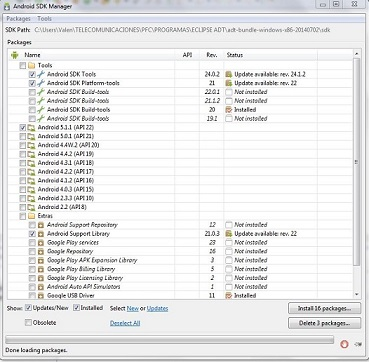
\includegraphics{imagenes/SDK.jpg}
			\caption{SDK Manager}
			\label{contexto:figura}
		\end{figure}
		
		A partir de aquí podremos escoger la versión API que deseamos instalar y con la cual trabajaremos para desarrollar nuestra aplicación. Debemos aceptar todo lo que contenga el paquete para que pueda ser instalado.
		
		Hay que destacar que SDK de Android y Eclipse son dos programas individuales, nada vinculados. SDK de Androis es la ventana que he mostrado en la imagen anterior y que como puede verse es un asistente de descargas. Mientras que Eclipse es la interfaz sobre la cual programaremos. Debemos vincularlos para poder programar en Android.
		
		Ahora trabajaremos con Eclipse, hay que vincular el SDK a nuestro entorno de desarrollo. Esto se realiza mediante la instalación de un plugin para Eclipse denominado ADT (Android Developent Tools). Tiene lógica que el plugin sean las herramientas de desarrollo de Android, ya que Eclipse como entorno de trabajo requiere de estas herramientas que no tiene para programar en Android.
		
		Este modo es un muy entretenido, por lo que recomiendo descargarse Eclipse ADT desde la página de Android Developers y evitar un trabajo extra.
		
		He de destacar que en este caso instalé la API de Android 4.4, ya que el dispositivo móvil en el que iba a probar la aplicación desarrollada dispone de dicha versión de Kernel de Android. Con ello evitaremos diferentes problemas de versión, además al no isntalar una de las últimas versiones de API de Android evitamos que surjan múltiples fallos a la hora de compilación o de versiones de Kernel.
		
		
	\newpage
	$\ $